\chapter{Исследовательская часть}

\section{Технические характеристики}
Характеристики используемого оборудования:
\begin{itemize}
    \item Операционная система --- Linux \cite{bib5}
    \item Память --- 16 Гб.
    \item Процессор --- AMD Ryzen 7 5800H \cite{bib6}
\end{itemize}

\section{Оценка алгоритмов}
В данном разделе оценку трудоемкости алгоритма будем дана в терминах числа сравнений, которые понадобились
для нахождения ответа. Размер массива равен $113$.

\medskip

Для алгоритма с полным перебором количество количество исходов равно длине массиве:
$n$ исходов, если элемент в множестве и еще один исход, когда элемент не в множестве.
Причем количество сравнений в худшем случае равно  $n$. Худший случай - это случай, когда
элемента или нет в множестве, или находится в самом его конце. Также
линейный поиск работает быстрее на отсортированном множестве, если
искомое значение лежит на индексе, примерно меньшем $\log_2(n)$. На рисунке
\ref{fig:images-Figure_1} представлена гистограмма алгоритма.

\begin{figure}[h]
    \centering
    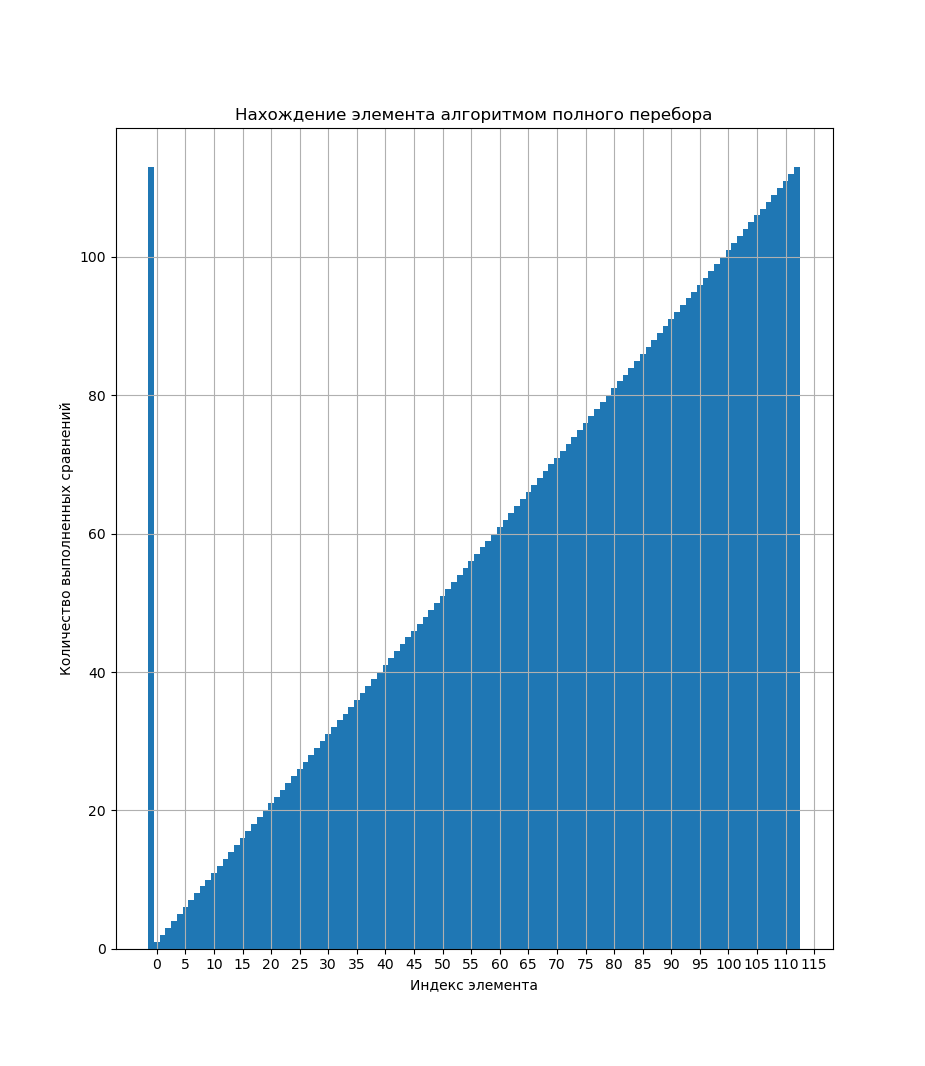
\includegraphics[width=0.8\textwidth]{images/Figure_1}
    \caption{Гистограмма алгоритма с полным перебором}
    \label{fig:images-Figure_1}
\end{figure}

\clearpage


Для алгоритма с двоичным поиском наибольшее количество сравнений не превышает
$log_2(n)$ в худшем случае. На рисунке
\ref{fig:images-Figure_2} и \ref{fig:images-Figure_3} представлены гистограммы алгоритма
двоичного поиска. На рисунке \ref{fig:images-Figure_3} изображена
гистограмма алгоритма с двоичным поиском, где количество сравнений
отсортировано по возрастанию.
\begin{figure}[h]
    \centering
    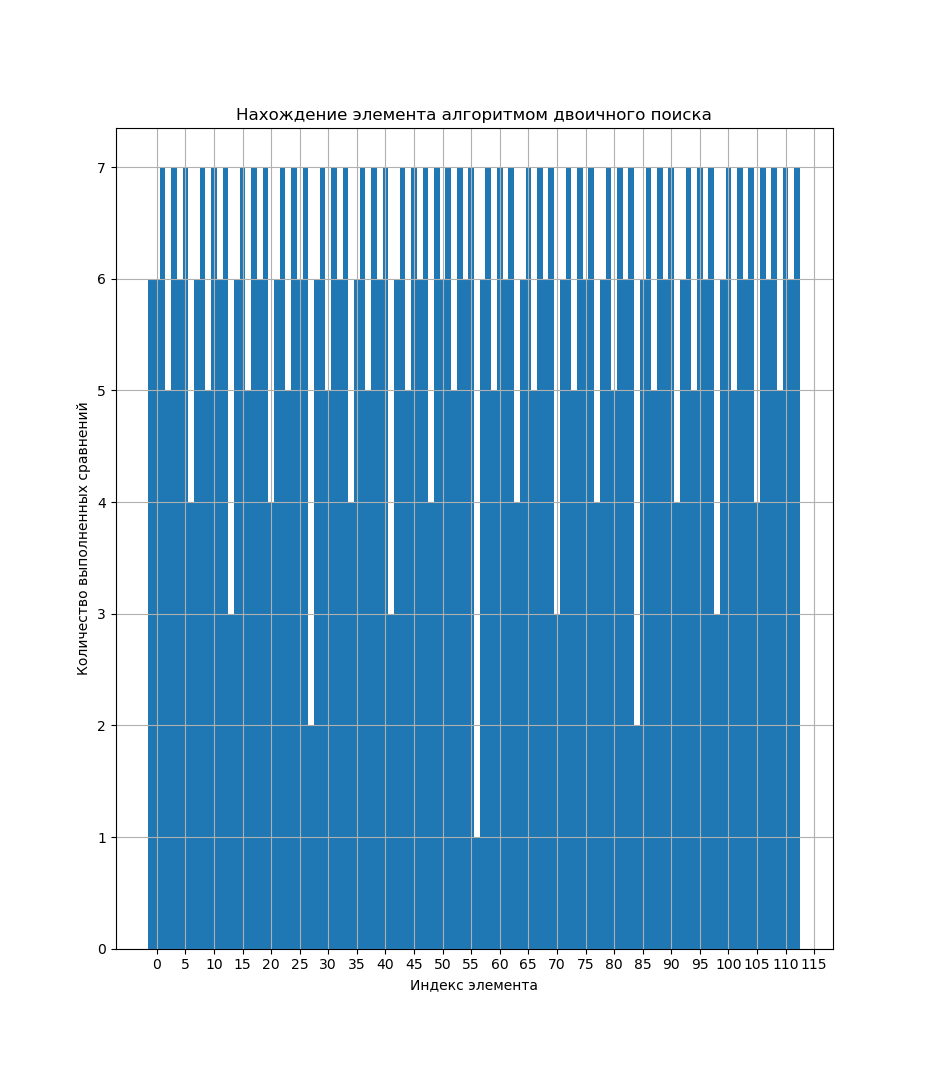
\includegraphics[width=0.8\textwidth]{images/Figure_2}
    \caption{Гистограмма алгоритма с двоичным поиском}
    \label{fig:images-Figure_2}
\end{figure}

\clearpage
\begin{figure}[h]
    \centering
    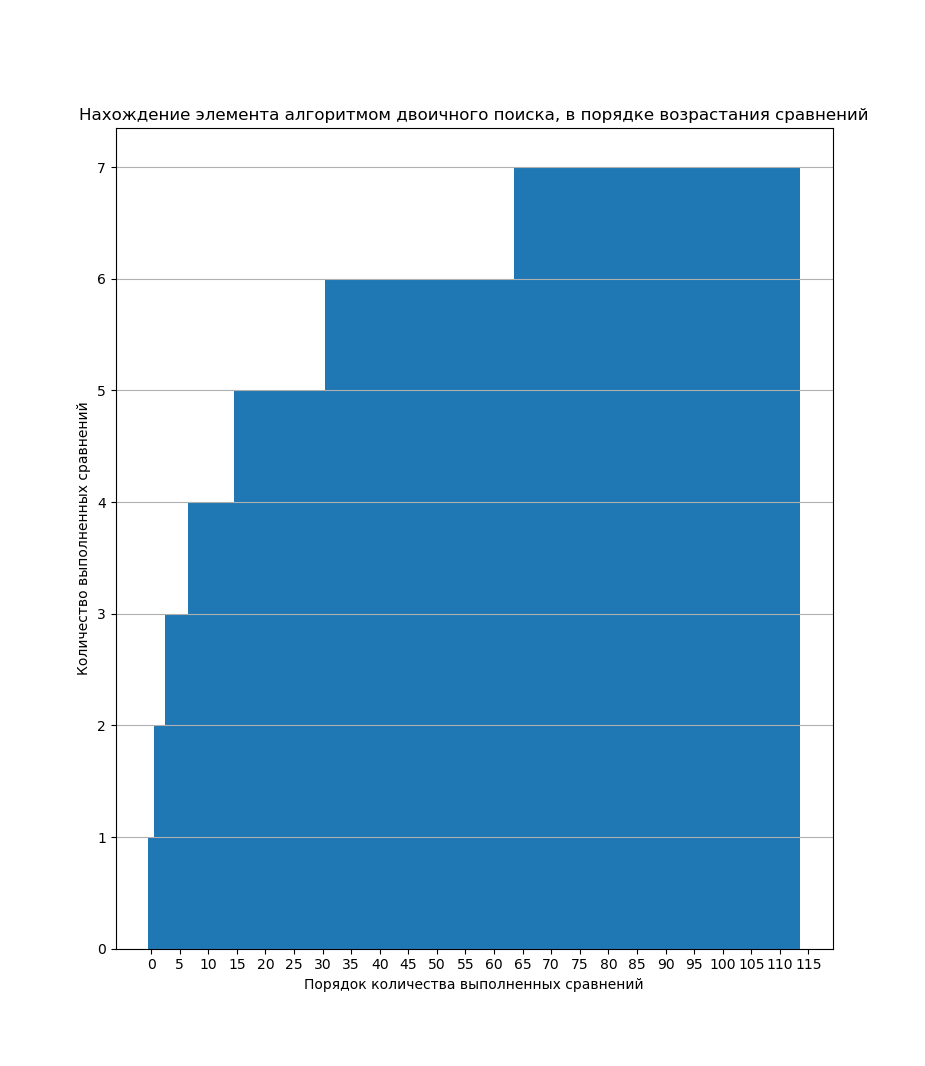
\includegraphics[width=0.8\textwidth]{images/Figure_3}
    \caption{Гистограмма алгоритма с двоичным поиском, отсортированная по количеству сравнений}
    \label{fig:images-Figure_3}
\end{figure}

\clearpage

\section{Вывод}

Для поиска заданного значения в массиве полным перебором количество сравнений растет
постепенно с увеличением индекса искомого элемента. Для поиска заданного значения
в массиве с помощью двоичного поиска количество сравнений в целом не зависит от
его расположения относительно начала и конца массива. Однако оно будет найдено быстрее, если лежит в середине массива, в четвертях и так далее.
Однако линейный поиск может работать быстрее бинарного поиска в случаях на отсортированном наборе,
если искомое значение примерно меньше индекса $\log_2(n)$, где $n$ --- размер набора. В случае,
если размер набора равен 113, то при индексах $1$ ---  $6$ линейный поиск быстрее работает, чем
двоичный поиск.

Наиболее эффективным алгоритмом является алгоритм с использованием двоичного поиска,
потому что количество сравнений в худшем случае не превышает $log_2(n)$, когда в алгоритме с
полным перебором количество в худшем случае равно $n$.

